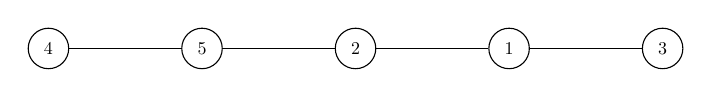
\begin{tikzpicture}[vertex/.style = {shape=circle,draw,minimum size=2.25em},scale=0.65, every node/.style={scale=0.65}]
    \node[vertex] (c1) at (0,0) {$1$};
    \node[vertex] (c2) at (-3,0) {$2$};
    \node[vertex] (c3) at (3,0) {$3$};
    \node[vertex] (c4) at (-9,0) {$4$};
    \node[vertex] (c5) at (-6,0) {$5$};
    \draw (c1) -- (c2);
    \draw (c1) -- (c3);
    \draw (c4) -- (c5);
    \draw (c2) -- (c5);
\end{tikzpicture}